\section{Task 1: Basic Probabilities and Visualizations }

\subsection*{$\xi$ values}

\begin{itemize}
    \item $\xi_1 = 1$
    \item $\xi_2 = 40$
\end{itemize}

\subsection{problem statement}

The number of meteorites falling into an ocean in a given year can be modeled by:

\begin{equation}

    P\left( x \right) = \frac{{e^{ - \xi_2 } \xi_2 ^x }}{{x!}}
\end{equation}

As seen in figure~\ref{fig:poisson}, the expected value of this distribution is $\xi_2$ and the median is $\xi_2$ too.

\begin{figure}[h]
\centering
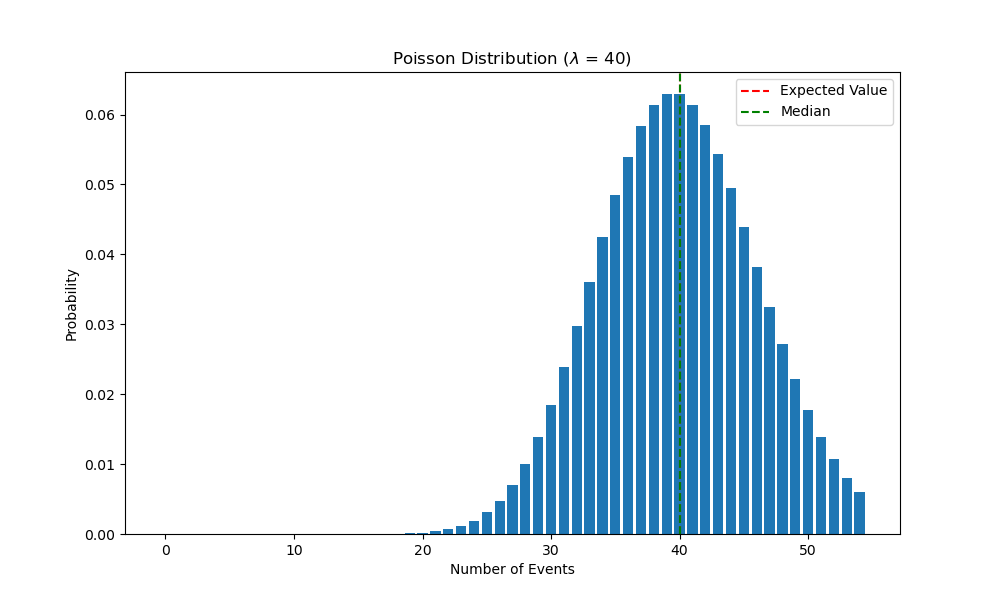
\includegraphics[width=8cm]{code/figures/poisson.png}
\caption{event distribution, with expected and median values\label{fig:poisson}
\end{figure}
\FloatBarrier

